%%%%%%%%%%%%%%%%%%%%%%%%%%%%%%%%%%%%%%%%%%%%%%%%%%%%%%%%%%%%%%%%%%%%%%%%%%%%%%%%
%2345678901234567890123456789012345678901234567890123456789012345678901234567890
%        1         2         3         4         5         6         7         8

\documentclass[letterpaper, 10 pt, conference]{ieeeconf}  % Comment this line out if you need a4paper

%\documentclass[a4paper, 10pt, conference]{ieeeconf}      % Use this line for a4 paper

\IEEEoverridecommandlockouts                              % This command is only needed if 
                                                          % you want to use the \thanks command

\overrideIEEEmargins                                      % Needed to meet printer requirements.

%In case you encounter the following error:
%Error 1010 The PDF file may be corrupt (unable to open PDF file) OR
%Error 1000 An error occurred while parsing a contents stream. Unable to analyze the PDF file.
%This is a known problem with pdfLaTeX conversion filter. The file cannot be opened with acrobat reader
%Please use one of the alternatives below to circumvent this error by uncommenting one or the other
%\pdfobjcompresslevel=0
%\pdfminorversion=4

% See the \addtolength command later in the file to balance the column lengths
% on the last page of the document

% The following packages can be found on http:\\www.ctan.org
\usepackage[pdftex]{graphicx}
\graphicspath{{figures/}{pictures/}{images/}}
\DeclareGraphicsExtensions{.pdf,.jpeg,.png,.eps}
%\usepackage{graphics} % for pdf, bitmapped graphics files
%\usepackage{epsfig} % for postscript graphics files
%\usepackage{mathptmx} % assumes new font selection scheme installed
%\usepackage{times} % assumes new font selection scheme installed
%\usepackage{amsmath} % assumes amsmath package installed
%\usepackage{amssymb}  % assumes amsmath package installed

\usepackage{here}
\usepackage{siunitx}

% \title{\LARGE \bf Presenting Force in Various Direction by Composing Force Vectors using Wearable Pin Matrix Display}
% \title{\LARGE \bf Presenting Force Distribution in Various Direction by Summing Paired Individual Forces from Fixed Pins of Finger-Mounted Pin-array Display}
\title{\LARGE \bf Presenting Force Distribution in Various Direction \\ using Pin-array Display}


\author{Takaaki Taniguchi$^{1}$, Yusuke Ujitoko$^{2}$, Sho Sakurai$^{3}$, Takuya Nojima$^{3}$, and Koichi Hirota$^{3}$% <-this % stops a space
% \thanks{*This work was not supported by any organization}% <-this % stops a space
\thanks{$^{1}$Takaaki Taniguchi is a Graduate Student of the University of Electro-Communications, Tokyo.
        {\tt\small takaaki16@vogue.is.uec.ac.jp}}%
\thanks{$^{2}$Yusuke Ujitoko is with Research \& Development Group, Hitachi, Ltd., Yokohama, Japan. and is a Graduate Student of the University of Electro-Communications, Tokyo.
        {\tt\small yusuke.ujitoko.uz@hitachi.com}}%
\thanks{$^{3}$Sho Sakurai, Takuya Nojima, Koichi Hirota is with the Graduate School of Information Systems, The University of Electro-Communications, Tokyo}}



\begin{document}



\maketitle
\thispagestyle{empty}
\pagestyle{empty}


%%%%%%%%%%%%%%%%%%%%%%%%%%%%%%%%%%%%%%%%%%%%%%%%%%%%%%%%%%%%%%%%%%%%%%%%%%%%%%%%
\begin{abstract}
This study proposes a novel method of presenting force distribution in various directions with the finger mounted pin-array display.
With the method, users feel the resultant force distribution by summing up the individual forces from paired-pins which tilted differently.
We hypothesize that we can control the direction and intensity of the resultant force by only changing the air pressure applied to each pin.
Two prototype devices are made to prove the concept.
The pin inclination of one device is fixed at 45$^{\circ}$ and that of the other device is fixed at 60$^{\circ}$.
We conducted two experiments.
The result of the first experiment shows that users could discriminate the direction of the force.
The discrimination accuracy was better with the 60$^{\circ}$ device than the 45$^{\circ}$ device.
The result of the second experiment shows that users could estimate the center of friction field by friction force distribution.
% Although all participants recognized the position of the friction field, there was an average variation of 3.75 mm between the center and their estimation. 
\end{abstract}

\section{INTRODUCTION}
% バーチャル物体を器用に扱う触覚デバイスは開発途上である
Today anyone can easily construct a virtual reality (VR) environment because of improvements in computer performance and advance in 3D technology such as head mount displays. 
Many VR technologies related to visual and auditory sensations are present in our surroundings and familiar in our lives.
However, the haptic device with which users can intuitively touch the virtual object, recognize the shape of it and dexterously operate it is still under research.

In order to reproduce the haptic information during the interaction between the finger and the virtual object, the haptic device should present the force distribution on the contact surface.
Depending on the shape of the object or frictional characteristics, not only the normal force but also the shear force should be presented to users.
As one of the approaches to reproduce the force distribution, the pin-array display has been developed ~\cite{Shimizu1993}~\cite{Koo2008}.
Though these pin-array devices could present force distribution, the direction of the force was fixed.
For example, most of them were able to present only normal force distributions~\cite{Moy2000,Velazquez2005,Sarakoglou2005,Kim2009}.

% 本研究では...

This study proposes a novel method of presenting force distribution in various directions with the finger mounted pin-array display, in which pins are tilted.
%We present users with the resultant force by summing up the individual forces from pins which tilted differently.
By pairing two pins tilted in different direction, it should be possible to present the resultant force of the two individual forces.
We hypothesize that we can control the felt direction of resultant force by only changing the air pressure applied to each pin (Fig.\ref{fig_intro}).
The method has two advantages.
First, the pin arrangement can be simple as previous pin-array devices and thus, the high density of pins is realized.
Second, it takes little time to change the pressure compared to changing the direction of the actuator itself and thus, the method can change of direction of the presented force with low latency.
We made a prototype system to prove the concept.
With this system, we evaluated how much users can discriminate the direction of the resultant force.
In addition, we conducted a user study where users found a force field resorting to frictional cue applied by the system.


% If the haptic information is accurately reproduced, the shape of the virtual object should be able to be conveyed to the user in the virtual environment.
% In order to reproduce the haptic information, various types of multi-contact-point haptic displays have been developed.
% This study focused on pin-array display type since it can provide robust force distribution on the surface of the virtual object.

% As the multi-point haptic displays, vibrotactile displays~\cite{Wang2006}, electrical displays~\cite{Kajimoto2014}, and pin-array displays~\cite{Shimizu1993}~\cite{Koo2008} have been developed.
% It is realtively easy to increase the contact point density with Vibrotactile displays and electrical displays.
% However, we consider that these methods are not suitable for shape presentation because they cannot present the robust pressure that occurs when touching a virtual object.
% On the other hand, pin-array displays are possible to reproduce the feeling of pressure since pins are pressed against the finger skin.
% Considering the reproducibility of the feeling of pressure, we focused on the pin-array display.

% pin arrayにも設置型と装着型の2種類ある。
% There are two types of pin-array display: grounded-type or wearable-type.
% The mechanically grounded pin-array display could present robust haptic cues using grounded forces with users~\cite{Shimizu1993, Howe, Leithinger:2010:RSA:1709886.1709928}.
% However, When users move the hand or finger to any position around users, these devices cannot display shapes.
% In other words, the workspace and portability are constrained.
% A large interactive mobile workspace may be useful for the exploration of virtual spaces.

\begin{figure}[t]
  \centering
  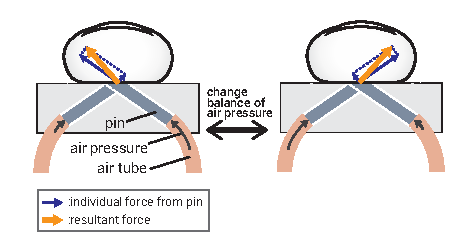
\includegraphics[width=3.4in]{images/fig_intro.eps}
  \caption{Proposed display presents the resultant force in various direction by summing individual forces from a pair of pins. We can change the direction of resultant force by only changing the air pressure on the air tubes.}
  \label{fig_intro}
\end{figure}

% 近年は装着型が多く開発されている
% Recently, more haptic system designs have started appearing with wearability in mind, and in this context wearable, pin-array displays have been developed~\cite{Koo2008, Kim2009}.
% However, currently, the ability to recognize the shape of virtual objects when using these wearable devices is worse than when users recognize real objects using a bare finger or hand.
% For example, our previous work by~\cite{taniguchi} evaluated shape recognition performance using a pin-array display covering the whole hand.
% The correct answer ratio was far inferior to the ones coming from the interaction between a real finger and the real objects, as obtained by~\cite{Klatzky1985}.

% shear方向の提示が形状認識に寄与すると思っている
% One of the promising approaches is to present not only normal force against surface but also shear force.
% The shear force should be essential for shape recognition since it provides frictional cues.
% There were studies that developed wearable display presenting shear force feedback such as \cite{Minamizawa:2007:GGW:1278280.1278289,6636291,Schorr:2017:FTD:3025453.3025744}.
% However, it is impossible to reproduce force distribution since these studies cause shear deformation of the whole skin using a pad.



\section{RELATED WORK}
\subsection{Grounded-type or Wearable-Type Pin-array Display}

% pin arrayにも設置型と装着型の2種類ある。
There are two types of pin-array display: grounded-type or wearable-type.
The mechanically grounded pin-array display could present robust haptic cues using grounded forces with users~\cite{Shimizu1993, Howe, Leithinger:2010:RSA:1709886.1709928}.
However, When users move the hand or finger to any position around users, these devices cannot display shapes.
In other words, the workspace and portability are constrained.
A large interactive mobile workspace may be useful for the exploration of virtual spaces.

% 近年は装着型が多く開発されている
Recently, more haptic system designs have started appearing with wearability in mind, and in this context wearable, pin-array displays have been developed~\cite{Koo2008, Kim2009}.
Thus, the present study focuses on these finger-mounted, wearable pin-array displays.

\subsection{Presenting Force Distribution using Pin-Arrays}

% 既存ピンアレイでは法線方向のみの提示が実現されてきた
Many researchers have developed pin-array display which can present users with force distribution feedback~\cite{Moy2000,Velazquez2005,Sarakoglou2005,Kim2009,Jang:2016:HED:2858036.2858264,Benko:2016:NTH:2984511.2984526}.
In order to provide more cutaneous cues, researchers have attempted to increase the denser pin-array display.
For example, Kim et al.~\cite{Kim2009} developed a wearable display composed of a $4\times8$ pin array on the fingertip.
The diameter of the pin was 0.5 mm, and the pins were arranged in a 1.5 mm interval.
The main focus of these previous studies existed on the simple structure of pin and actuators for denser pin arrangements.
In contrast, the increase in the degree of freedom of force feedback has not been paid attention to.
For example, most of them were able to present only normal force distributions.


\subsection{Presenting Force in Various Direction}

% でも接線方向も大事
Although the presentation of force in the normal direction is important in communicating contact with the object, in order to realize the more natural interaction close to reality with the virtual object, it is also necessary to present the force in shear direction caused by friction.

% 接線方向にも力を提示できるディスプレイが開発されている。
% しかし一方向の力しか提示できず力の分布は提示できない
There were studies that developed display presenting shear force feedback.
For example, Minamizawa et al.~\cite{Minamizawa:2007:GGW:1278280.1278289} developed a method of laterally displacing the pad pressed against the finger by the force of the actuator in two-dimension. 
The work by ~\cite{6636291,Schorr:2017:FTD:3025453.3025744} extended it to three-dimension and their display moved the pad three degrees of freedom.
However, it is impossible to reproduce force distribution since these studies cause shear deformation of the whole skin using a pad.

This study develops the finger-mounted pin-array display which presents force distribution in various directions.



\section{CONCEPT AND PROTOTYPE DEVICE}

\subsection{Concept}

As stated in the Introduction section, this study proposes a new concept of present force distribution using only fixed, tilted pin-arrays.
The resultant force vector can be calculated based on the pin's inclination angle and intensity of individual force of from two pins as follows (shown in Fig.\ref{fig_stimulus}) :

\begin{figure}[h]
  \centering
  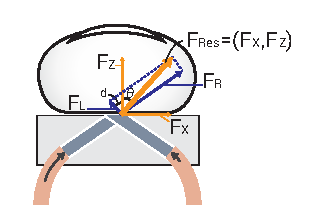
\includegraphics[width=2.0in]{images/fig_stimulus}
  \caption{Resultant force vector can be calculated by the pin's inclination angle and individual force intensity of from two pins.}
  \label{fig_stimulus}
\end{figure}


\begin{equation}
\label{eq:1}
\left(
\begin{array}{c}
F_{X} \\
F_{Z} \\
\end{array}
\right)
= 
\left(
\begin{array}{cc}
-\sin{d} & \sin{d} \\
\cos{d} & \cos{d} \\
\end{array}
\right)
\left(
\begin{array}{c}
F_{L} \\
F_{R} \\
\end{array}
\right)
\end{equation}

\begin{equation}
\label{eq:theta}
% \tan{\theta} = \frac{F_{X}}{F_{Z}}
\theta = \arctan{ \frac{F_{X}}{F_{Z}} }
\end{equation}

where $F_{Res} = (F_{X}, F_{Z})$ is the intensity of the resultant force, $\theta$ is the inclination angle of resultant force, $F_{L}$, $F_{R}$ are the intensity of individual force from each pin, and $d$ is the inclination angle of the pin.
We can solve the expression in terms of pin's intensity as follows:

\begin{equation}
\label{eq:2}
\left(
\begin{array}{c}
F_{L} \\
F_{R} \\
\end{array}
\right)
= 
\frac{1}{2\cos{d}\sin{d}}
\left(
\begin{array}{cc}
\cos{d} & \sin{d} \\
-\cos{d} & \sin{d} \\
\end{array}
\right)
\left(
\begin{array}{c}
F_{X} \\
F_{Z} \\
\end{array}
\right)
\end{equation}

According to (\ref{eq:2}), we can define the pin's output intensity $(F_{L}, F_{R})$ based on the pin's angle $d$ and the intensity of resultant force $(F_{X}, F_{Z})$.
We can control $F_{R}$, $F_{L}$ by only changing the air pressure for each pin.
On the other hand, we need to consider what value of $d$ is the best.
We made two prototype devices that had different inclination angles of $d$ and evaluate them through the user study.

\subsection{Prototype Device}

We made a prototype pin-array display device.
This device has a simple structure with holes in the base.
As shown in Fig. \ref{fig_intro}, the holes tilted to the left and the right to make a pair.
A 2.0 mm diameter pin is set in the hole.
This pin is driven like an air cylinder and functions as an actuator that compresses the skin.
The pin is driven by air pressure.
By defining the pneumatic output to the pin tilted to the right ($F_{R}$) and the left ($F_{L}$), the x and y components of the resultant force ($F_{X}$, $F_{Z}$) are determined.
After all, by changing the intensity of the air pressure output to each of the left and right pins, it is possible to change the direction and strength of the resultant force outputted by the pair of pins.
There are two types prototype.
We refer to the display where pins tilted 45${\circ}$ as "45$^{\circ}$ device".
We call the other display "60$^{\circ}$ device".
Next, we describe each device in detail.

%Both devices had 18 (=$3\times6$) holes with a diameter of 2 mm on the surface.
%The pins were set in the holes.
%Each pin was actuated by the air cylinder, which was controlled by the regulator from the remote.
%The pins were tilted 45$^{\circ}$ or 60$^{\circ}$.
%We refer to the display where pins were tilted 45$^{\circ}$ as "45$^{\circ}$ device".
%We call the other display "60$^{\circ}$ device".
%In both devices, the nine out of all pins were tilted to the right and the remaining nine pins were tilted to the left. 
%The pin tilted to the right and the pin tilted to the left intersected each other, and thus they forming nine pairs. 
%By changing the intensity of the air pressure output to each of the left and right pins, it was possible to change the direction and strength of the resultant force outputted by the pair of pins. Next, we describe each device in detail.


\subsubsection{45$^{\circ}$ Device}

%ピンの断面積6.1mm^2
Fig.\ref{fig_45_device} (a)~(c) shows the structure of the 45$^{\circ}$ device. 
As shown in Fig.\ref{fig_45_device} (a), (c), the tilt angle of the pins was 45$^{\circ}$. 
% Nine pins were tilted to the right and the remaining nine pins were tilted to the left. 
%Two pins that were tilted to the right and the left made a pair (Fig.\ref{fig_45_device}(b)). 
There were nine pairs with the $3\times3$ arrangement (Fig.\ref{fig_45_device}(b)).
We refer to the interval between centers of the two holes as pin pitch.
The pitch of the paired pins was 3.9 mm.
The pitch between the pins on the same row was 5.0 mm. 
%We 3D printed the base with polyacetal and connected air tube to the hole.
The device was implemented with a polyacetal substrate by a computerized numerical control (CNC) milling machine.
% and the small rubber pad is set on each pin.
The upper part of the pin was cut at 45$^{\circ}$ to flatten the device surface, and the cross-sectional area was 6.1 $mm^2$.
%ピンの上部をカットした話と,その断面積についての記述
An air tube for sending air was connected to the bottom of the hole where the pin was set.

%Fig. \ref{fig_45_device} (d) shows the appearance of the device.

\begin{figure}[h]
  \centering
  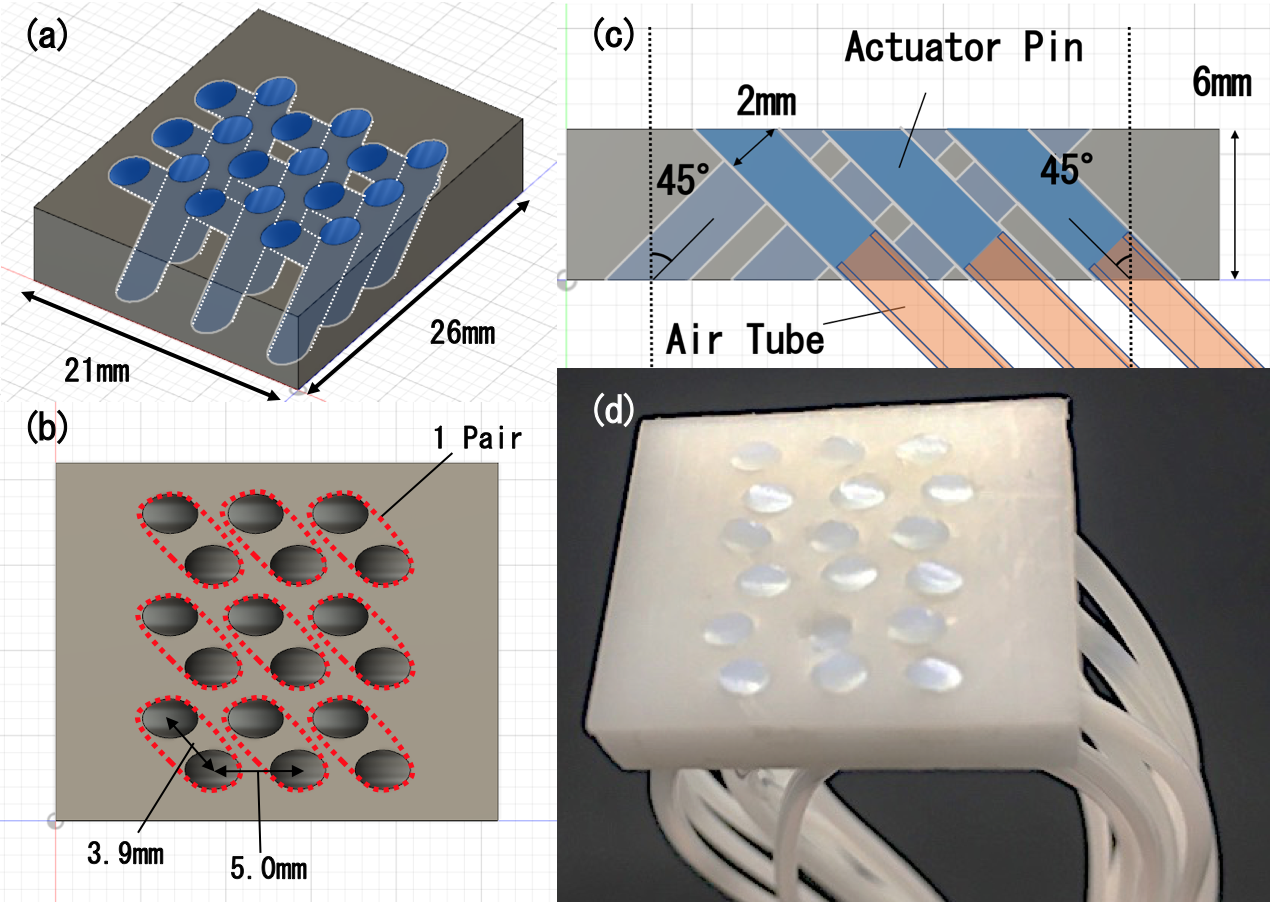
\includegraphics[width=3.4in]{images/fig_45_device}
  \caption{45$^{\circ}$ device.
(a)Design, (b)Nine Pairs of the pins tilted to the right and the left, 
(c)Cross section, (d)appearance
}
  \label{fig_45_device}
\end{figure}

\subsubsection{60$^{\circ}$ Device}
%ピンの断面積8.3
The pins were tilted 60$^{\circ}$ to the right and the left.
%The pins tilted to the right and the pins tilted to the left formed nine pairs. 
There are 9 pairs of the pins as well as 45$^{\circ}$ device.
The internal structure and implementation of the device are shown in Fig.\ref{fig_60_device} (a)~(d).
The pitch of the paired pins was 3.0 mm.
The pitch between the pins on the same row was 6.6 mm.
Like the 45$^{\circ}$ device, the 60$^{\circ}$ device implemented with a polyacetal substrate by a CNC milling machine.
The top of the pin was cut at 60$^{\circ}$ to flatten the device surface, and the cross-sectional area was 8.3 $mm^2$.
%ピンをカットした話とその断面積の記述.
An air tube for sending air was connected to the bottom of the hole where the pin was set.

\begin{figure}[h]
  \centering
  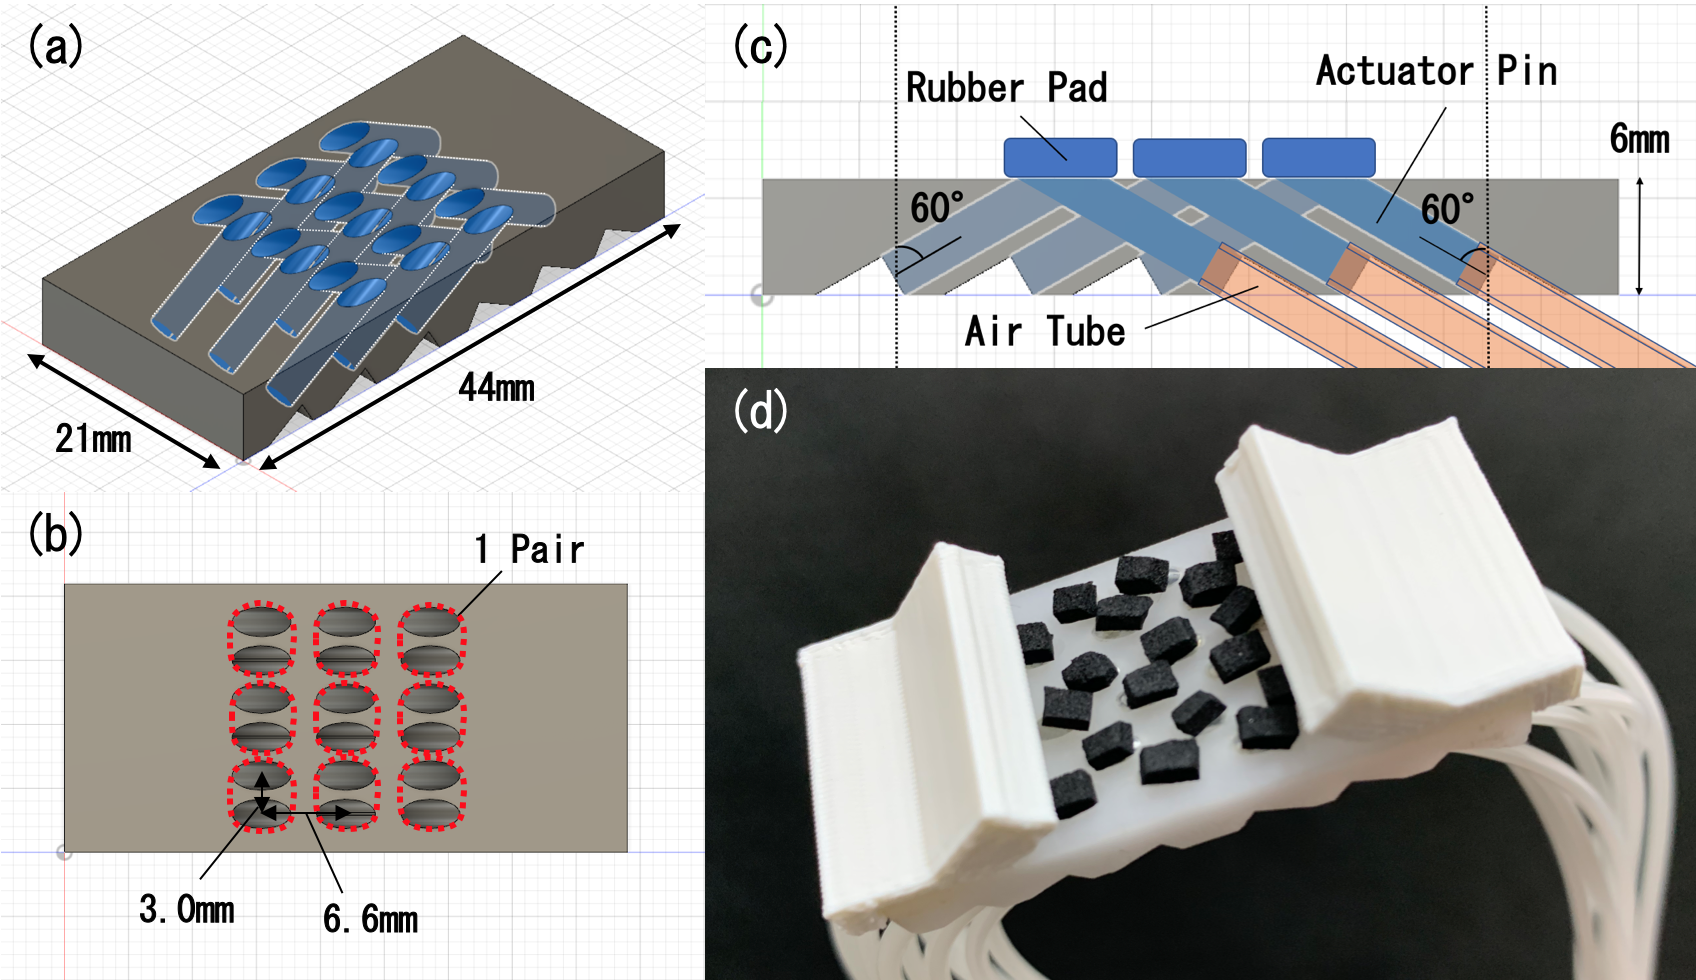
\includegraphics[width=3.4in]{images/fig_60_device}
  \caption{60$^{\circ}$ Device
(a)Design, (b)Nine Pairs of the pins tilted to the right and the left,
(c)Cross section, (d)Appearance}
  \label{fig_60_device}
\end{figure}

%The space between the pins on the same row was 2.0 mm, and the 0.7 mm on the same columns. 
% However, due to the accuracy of the machine tool, the implemented device had a deviation of 3mm between the holes of the pins tilted to the right and the left (Fig. 2 (d)). %これは蛇足感

In the 60$^{\circ}$ device, two attachments were newly adopted as compared to the 45$^{\circ}$ device.
The first attachment was a rubber pad equipped to the top of the pin (Fig.\ref{fig_60_device} (b)).
This rubber pad made it possible to cause shear skin deformation by enhancing the friction between the skin and the pad. 
The second attachment was support parts that fixed the finger to which the device is attached (Fig.\ref{fig_support_parts}).
This support part prevented the side slip of the finger position that was caused by the tangential pressure due to the pin. 

\begin{figure}[h]
  \centering
  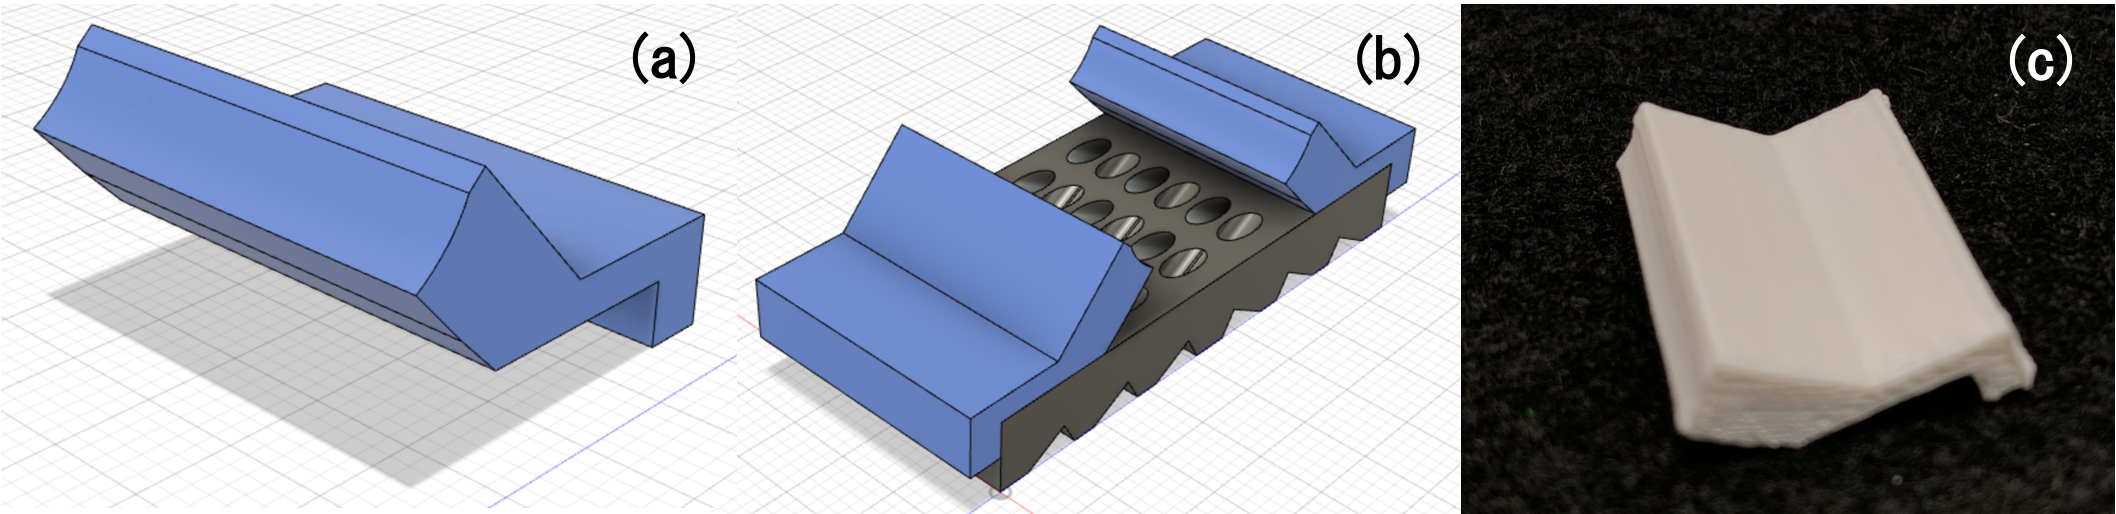
\includegraphics[width=3.4in]{images/fig_support_parts.png}
  \caption{Support Parts
(a)Design, (b)Mounted support parts, (c)Appearance}
  \label{fig_support_parts}
\end{figure}

\subsubsection{Control System}

Block diagram of the system shown in Fig.\ref{fig_block_diagram}.
This system was composed of electro-pneumatic regulators, the control circuit, and the PC. The pressure of the air was regulated by the electro-pneumatic regulator and was transmitted to each actuator via the air tube. 
The output pressure of the regulator was commanded by the PC (controller PC) through the control circuit.

\begin{figure}[h]
  \centering
  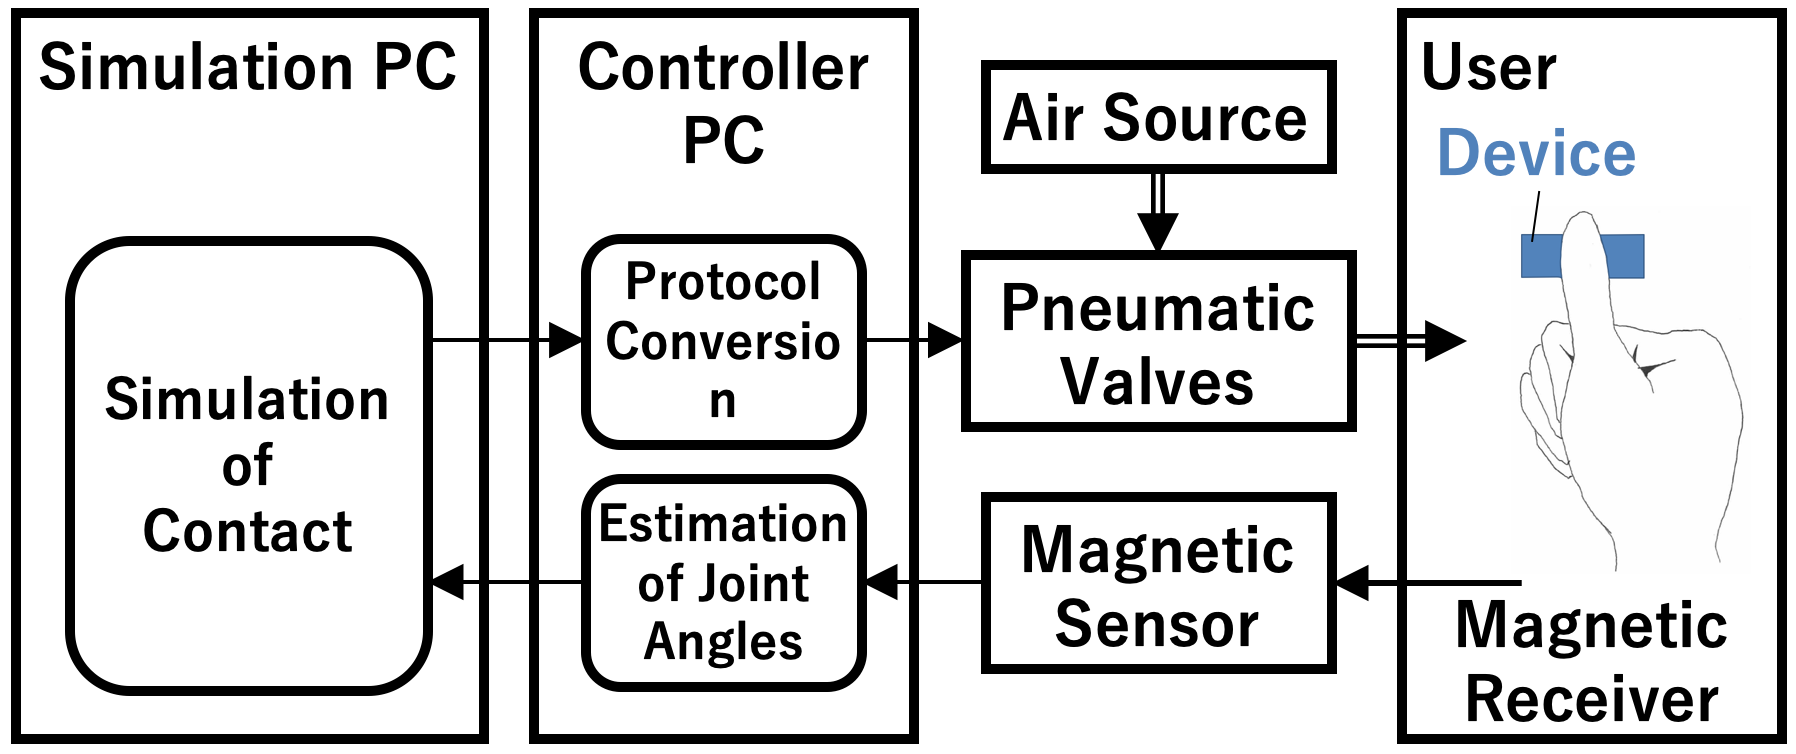
\includegraphics[width=3.4in]{images/fig_block_diagram.png}
  \caption{Block Diagram of The Control System}
  \label{fig_block_diagram}
\end{figure}

\section{EXPERIMENT 1: DISCRIMINATING DIRECTION OF RESULTANT FORCES}

%In this experiment, we evaluated whether the direction of the resultant force from the device was perceived correctly.
In this experiment, we evaluated whether the direction of the tangential force presented by the device was perceived correctly.
Participants answered the direction of force either left or right.
%The experiment was designed by following a just noticeable differences (JND) methodology~\cite{gescheider1985psychophysics}. 
The experiment was performed by a constant method, and a psychometric curve was obtained as a result of discriminating the direction perceived by the participants.

\subsection{Experimental Environment}

Participants sat on a chair, and they wore either 45$^{\circ}$ or 60$^{\circ}$ device on their fingertip of the dominant hands'{} thumb. 
During the experiment, participants wore the headphone with noise canceling function, and environmental noise was blocked by white noise from the headphone.
Fig.\ref{fig_ex1_environment} shows an experimental environment of experiment 1. 
The number of participants was eight (six males and two females, aged between 22 to 26).

\begin{figure}[h]
  \centering
  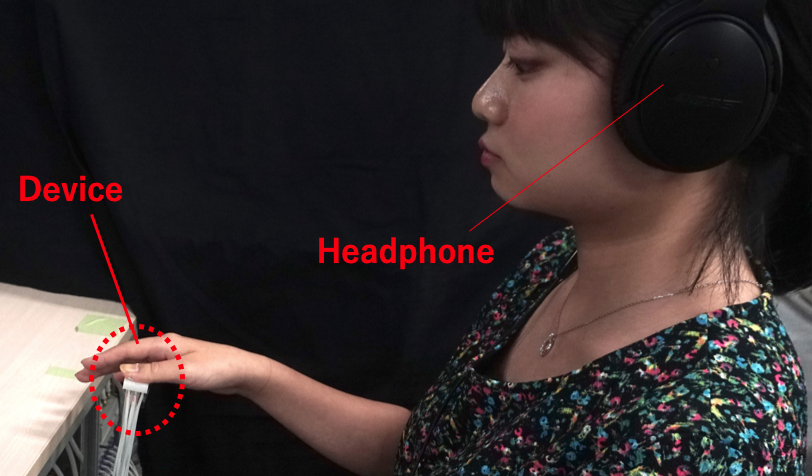
\includegraphics[width=3.4in]{images/fig_ex1_environment.png}
  \caption{Experimental environment of the experiment 1.}
  \label{fig_ex1_environment}
\end{figure}

\subsection{Standard Stimulus and Comparison Stimuli}

Standard stimulus was the stimulus when $\theta$ was 0$^{\circ}$ in expression (\ref{eq:theta}). % 圧力がどれくらいだったかの記述が必要
% A. 式(1)の結果が1Nになるように圧力を決定
% 標準刺激の場合は45dデバイスで0.116Mpa, 60dデバイスで0.120Mpaですね.→ありがとうございます!
%The pressure output to each pin of the standard stimulus was 0.116 Mpa for the 45$^{\circ}$ device and 0.120 Mpa for the 60$^{\circ}$ device.
%These values were configured so that the intensity of the resultant force in expression (\ref{eq:1}) equaled to 1N.
 The pressure output $F_{R}$ and $F_{L}$ were designed so that the resultant force in expression (\ref{eq:1}) equaled to 1N.

On the other hand, the comparison stimulus was the stimulus $\theta$ of which was every 5$^{\circ}$ from the limit angle that each device can present. 
In the case of the 45$^{\circ}$ device, the comparison stimulus was the ones when $\theta$ was from +45$^{\circ}$ to -45$^{\circ}$. 
In the case of 60$^{\circ}$ device, the comparison stimulus was the ones when $\theta$ was from +60$^{\circ}$ to -60.
% As the angle of the force of the presentation stimulus tilts from 0$^{\circ}$, the direction becomes easier to perceive.
% Therefore, it is considered that the correct answer rate becomes higher as the angle becomes larger. % ここに仮説を書くかはあとで考える。

\subsection{Task Design}

For each trial, participants performed
the standard stimulus and the comparison stimulus sequentially, and they stated whether the direction of the tangential force presented from the device was "left" or "right". % 刺激した時間ってどのくらい?
% A. 標準刺激は約1秒くらい提示しました.
%    比較刺激の方は被験者が答えるまで無制限で出してました.
%    大体の被験者は2,3秒で答えてましたが,たまに迷った時は5秒くらいかかってたときもありました.
%    ただ時間的な記録が残っていないので,無制限としか書けないですね.
Standard stimulus was presented for about 1 second.
The comparison stimulus continued to be presented until participants answered.

For each comparison stimulus, the participant answered 5 times. % 試行回数いくつだっけ
%A. 5回です.
With 45$^{\circ}$ device, the number of comparison stimuli was 18 and thus, the total number of trials per participant was 90. 
With 60$^{\circ}$ device, the number of comparison stimuli was 24 and thus, the total number of trials per participant was 120. % 広田先生に冗長といわれるかも
The order of comparison stimuli was randomly assigned.
In addition, whether participants wore 45$^{\circ}$ or 60$^{\circ}$ device first was assigned to the participant to be counter-balanced.

\subsection{Results}

Fig.\ref{fig_jnd_45} and Fig.\ref{fig_jnd_60} show the average value of the probability that the participants answered “right”. 
Error bars represent standard error. 
The ratio of answering “right” increased as the angle leaned further to right in both devices. 
%In order to investigate the subjective equivalent point and the discrimination thresholds for clearly recognizing the difference in angles, the least-squares fitting was performed using a cumulative normal distribution function, which is shown in the orange line in Fig.\ref{fig_jnd_45} and Fig.\ref{fig_jnd_60}.
In order to obtain a psychometric curve, the least-squares fitting was performed using a cumulative normal distribution function, which is shown in the orange line in Fig. \ref{fig_jnd_45} and Fig. \ref{fig_jnd_60}.
The point of subjective equality (PSE), which represents the value of evaluation stimulus judged as “equal to the standard stimulus”, was +3.1$^{\circ}$ in the 45$^{\circ}$ device and +4.3$^{\circ}$ in the 60$^{\circ}$ device. 
The just-noticeable difference (JND) representing “the minimum difference between 2 stimuli discrimination with a confidence rate of 50\% of the judgment number” was 46.5$^{\circ}$ in the 45$^{\circ}$ device and 36.4$^{\circ}$ in the 60$^{\circ}$ device.

\begin{figure}[h]
  \centering
  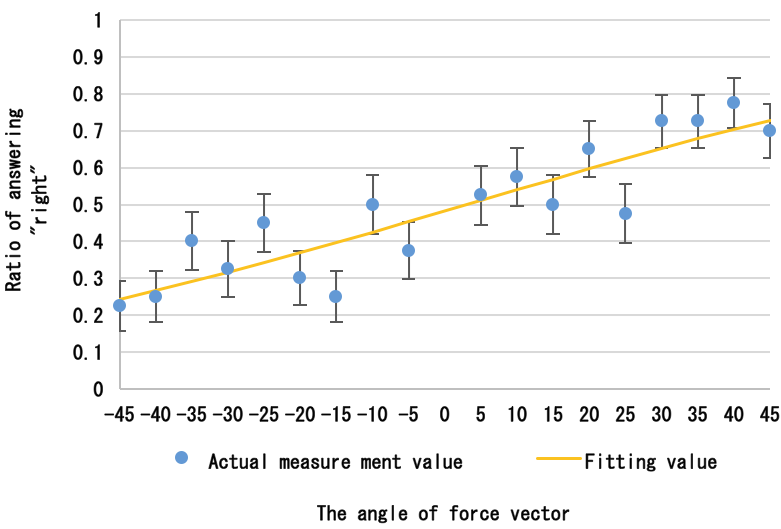
\includegraphics[width=3.4in]{images/fig_jnd_45.png}
  \caption{The ratio of participants answer "right" with the 45$^{\circ}$ device.}
  \label{fig_jnd_45}
\end{figure}

\begin{figure}[h]
  \centering
  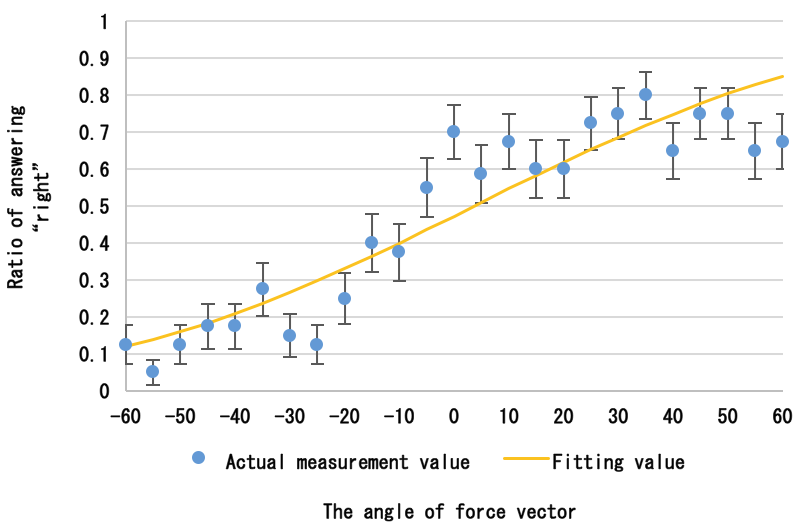
\includegraphics[width=3.4in]{images/fig_jnd_60.png}
  \caption{The ratio of participants answer "right" with the 60$^{\circ}$ device.}
  \label{fig_jnd_60}
\end{figure}

\subsection{Discussion}
%According to the result, participants discriminated the direction of resultant force at approximately 75\% at maximum with 45$^{\circ}$ device and 85\% at maximum with 60$^{\circ}$ device.
%Thus, the discrimination performance was better with 60$^{\circ}$ device than 45$^{\circ}$ device.
%The comparison between the JND value suggests the same conclusion.
%This is reasonable because the cosine term becomes large when $d$ is large in expression (\ref{eq:1}).

%被験者ごとのJNDをt検定で比較したが有意差なし
In this experiment, the JND of the 60$^{\circ}$ device was smaller than 45$^{\circ}$ device.
To determine whether there is a difference in the JND of two conditions, we performed the t-test obtained from each participants'{} JND values.
However, there was no significant difference.

%To realize better performance, the increase in the pin's inclination angle is one option.

%有意差はないが,60dデバイスの方が提示可能な刺激の角度が30度多い.
%(左右に15度ずつ)
%そのため,ピンの傾斜角を増加させることは,提示可能な刺激の自由度を高めることにつながる.
%Although there was no significant difference in the JND, 60$^{\circ}$ device can present 30$^{\circ}$ (15$^{\circ}$ left and right) larger angles than the 45$^{\circ}$ device.
There was no significant difference in the JND which suggests that the 60d device is a better implementation in that it can prezent the force of wider angle range.
Thus, increasing the pin's inclination angle will increase the degree of felt inclination of the angle of the resultant force that the device can present.

Another option to increase the felt inclination angle of the resultant force will be to increase the number of pins or applied pressure.
We should flexibly change these parameters based on design constraints to realize better recognition performance.

Overall, we showed that there is a possibility that participants can recognize the direction of the resultant force with the proposed device.

\section{EXPERIMENT 2: RECOGNITION OF THE FRICTION FIELD LOCATION}

%Unlike the previous experiment where the resultant force vector of all pins was the same, 
In this experiment, the recognition of force distribution was investigated.
We assumed a field in which the friction coefficient varies in a distributed manner.
The distribution follows the cosine function and is largest at the center and smaller with distance from the center.
Participants were asked to find the center of the frictional field on the virtual surface.
Participants wore the device and explored the surface and found the position by resorting to frictional force distribution provided by the device.

The number of participants was five (four males and one female, aged between 23 to 26).

\subsection{Experimental Environment}

In this experiment, only the 60$^{\circ}$ device was used. 
This is because the 60$^{\circ}$ device has the smaller JND than the 45$^{\circ}$ device.
As in Experiment 1, participants sat on a chair and explore the surface with the device. 
The position of their finger was measured using a magnetic sensor and it was sent to the simulation. 
During exploration, participants could see the display the position of the virtual finger on the virtual surface on display. Blue nodes corresponded to the pair of pins (Fig.\ref{fig_experimental_window}).

% We recorded the center coordinates of the participant finger. 

\begin{figure}[h]
  \centering
  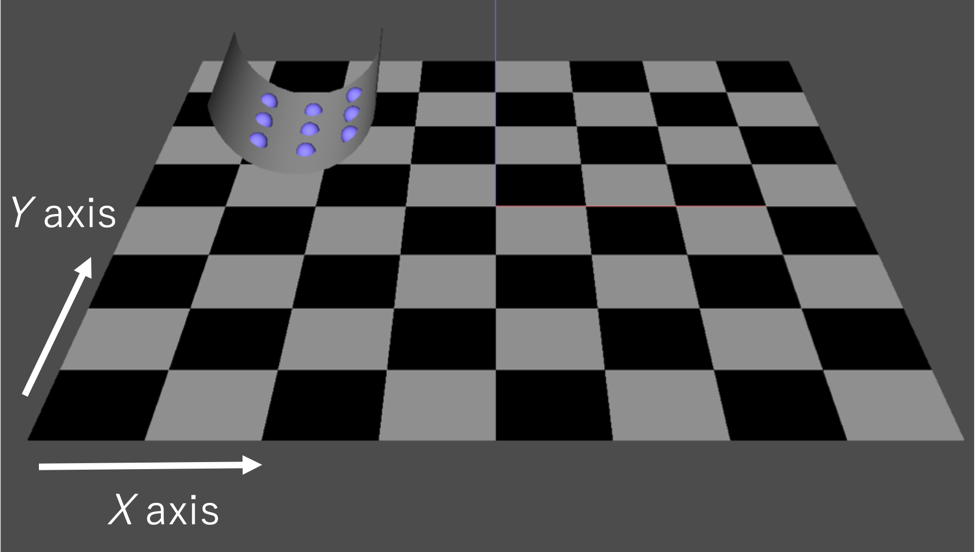
\includegraphics[width=2.9in]{images/fig_experimental_window.png}
  \caption{Participants watched the position of virtual finger on virtual surface. Blue nodes corresponded to the pair of pins}
  \label{fig_experimental_window}
\end{figure}

We designed a "friction field" in which friction coefficient varies in a distributed manner with a radius of 20 mm on the virtual surface with 80mm $\times$ 80mm.
Nine center coordinates of the friction field visualized in black in Fig.\ref{fig_friction_position} were prepared. 
One of them is visualized in red in Fig.\ref{fig_friction_position}. 

\begin{figure}[h]
  \centering
  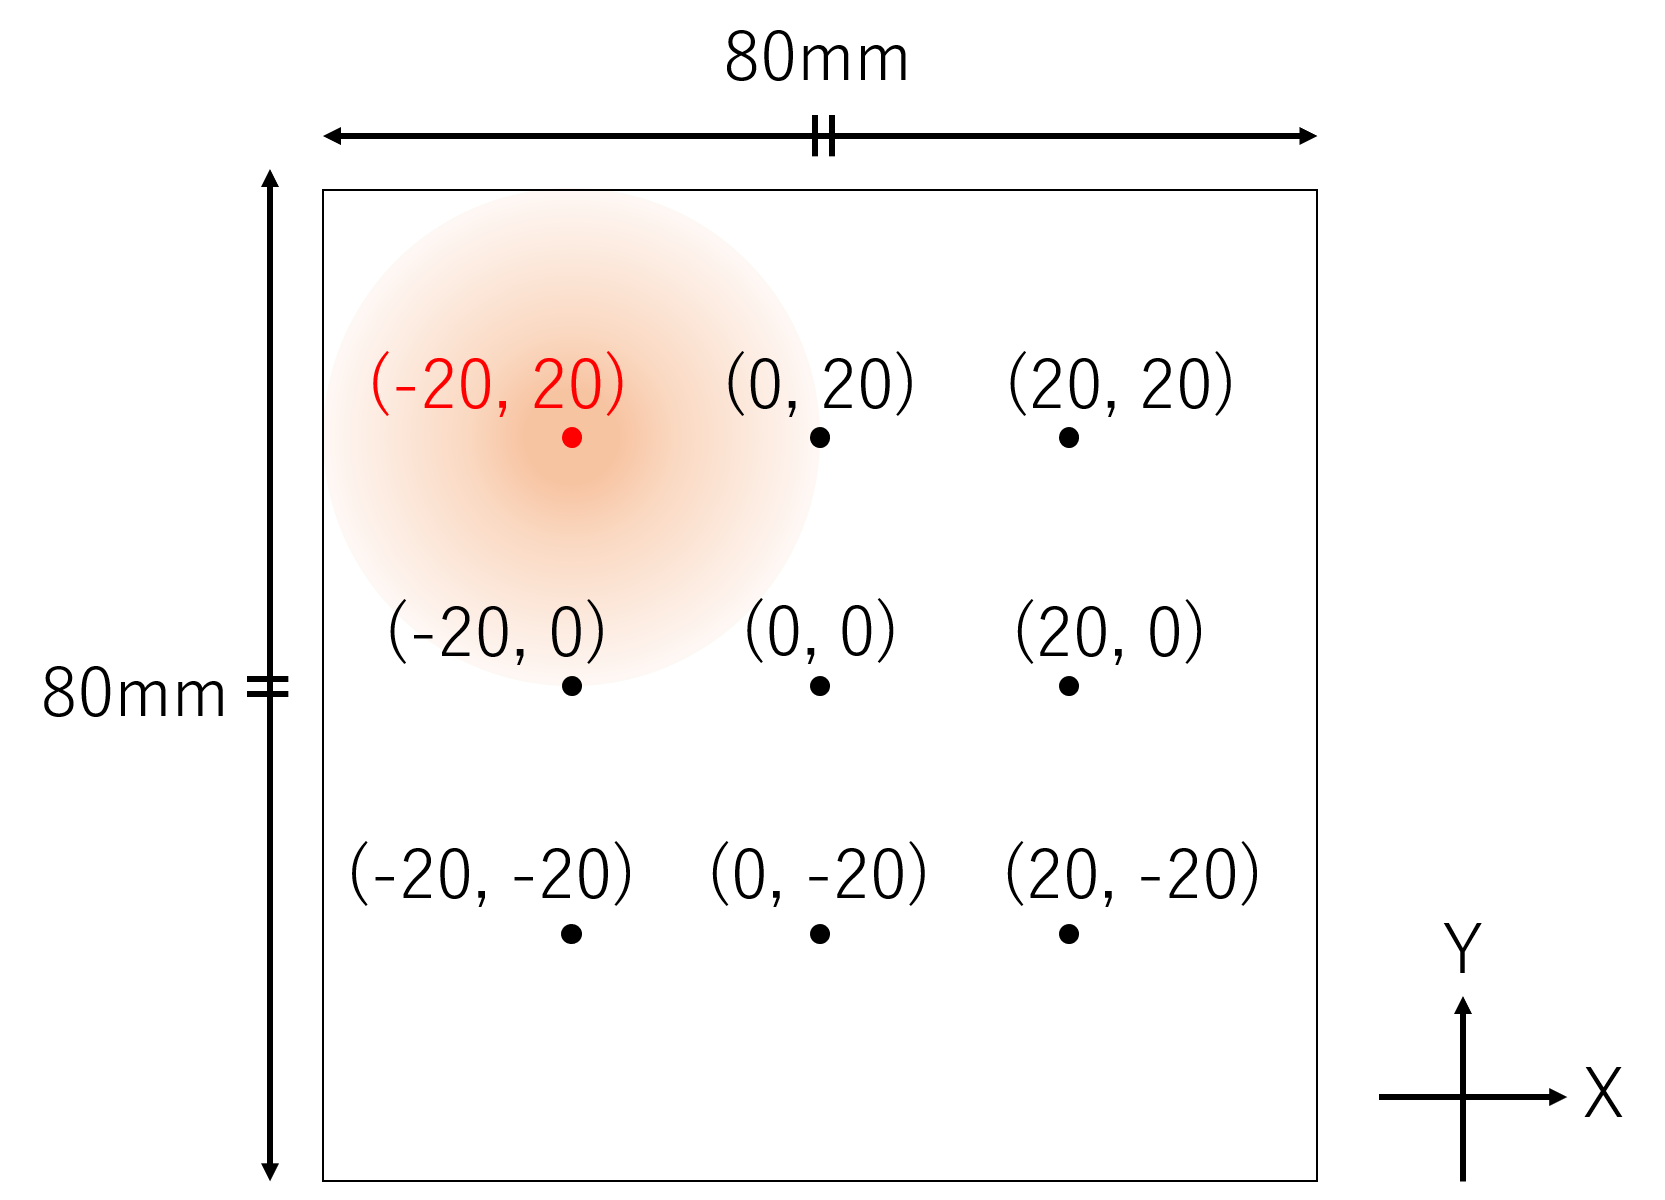
\includegraphics[width=2.1in]{images/fig_friction_field}
  \caption{Nine candidate of center coordinate of friction field. One of the friction field is visualized.}
  \label{fig_friction_position}
\end{figure}

% The friction coefficient of the friction field varied depending on the distance from the center.
The friction coefficient was 1 at the center and its value decreased from the center towards the outside. 
It was determined by the following formula:

\begin{equation}
    \mu = (\cos{\frac{\pi r}{2 radius}})^2
\end{equation}

where $\mu$ is the friction coefficient at that coordinate. 
$r$ is the distance from the center of the friction field (mm), and $radius$  is the radius of the friction field (20 mm).
$\mu$ defined the resultant force ($F_{X}$, $F_{Z}$) as follows:

\begin{equation}
\label{F_z}
    F_{Z} = k \cdot \Delta z 
\end{equation}
\begin{equation}
\label{F_x}
    F_{X} = - \mu \cdot \mathrm{sgn}(v) \cdot k \cdot \Delta z
\end{equation}

where $v$  is the direction component of the finger obtained by dividing the velocity vector by the absolute velocity value, $k$ is the elastic modulus (0.1), and $\Delta z$ is the distance penetrated by the finger into the virtual surface (mm). 
The force output to each pin $F_{R}$, $F_{L}$ of the device is determined by expression (\ref{F_x})(\ref{F_z}), and (\ref{eq:2}).

\subsection{Task Design}

The experiment consisted of a practice phase and an evaluation phase. 

In the practice phase, participants could feel the frictional cue in order to familiarize themselves with the operation of the device only once.
After that, the evaluation phase was carried out.
In the evaluation phase, participants were instructed to find the center of the friction field.
Participants could freely move their index finger with the device on the surface without a time limit.
When they found the center, they put their thumb on it and pushed the button of the keyboard.
Participants were instructed to search with the thumb orientation fixed in the $Y$ axis direction.
% Also, Participants explored while looking at the positional relationship between their fingertip and the floor (Fig. 9 (a)).  % ちょっとよくわからなかった..

The trials of exploration were conducted 36 times, nine center coordinates of the friction field were prepared and randomly determined.

\subsection{Data Analysis}

We preprocessed the obtained data to compensate individual differences of the center coordinate of their fingertips.
We assume that the mean value of the responses for each participant was the center coordinates of the participant’s fingertips.
Thus, we obtained the compensated value by subtracting the value from each answer value for each participant. 
We performed a single round of 3$\sigma$ clipping to remove
outliers. 
The following analysis was performed on the data that did not include outliers.

With this device, with regard to the $X$ axis, participants received frictional cues as shear and normal force distribution expressed in equation (\ref{F_x}) and (\ref{F_z}) respectively.
%In contrast, with regard to the $Y$ axis, participants only received normal force distribution in expression (\ref{F_z}).
While, with regard to the $Y$ axis, no tangential component caused by the friction was presented.
To determine whether there is a difference in error along $X$ and error along $Y$ axes, we conducted the t-test per participant.

\subsection{Result}

\begin{figure}[h]
  \centering
  \includegraphics[width=3.0in]{images/fig_ex2_res}
  \caption{Recorded fingertip coordinates of each participant (mm).}
  \label{fig_ex2_res}
\end{figure}

\begin{table}[h]
  \centering
  \caption{Standard deviation of each participant (mm).}  
  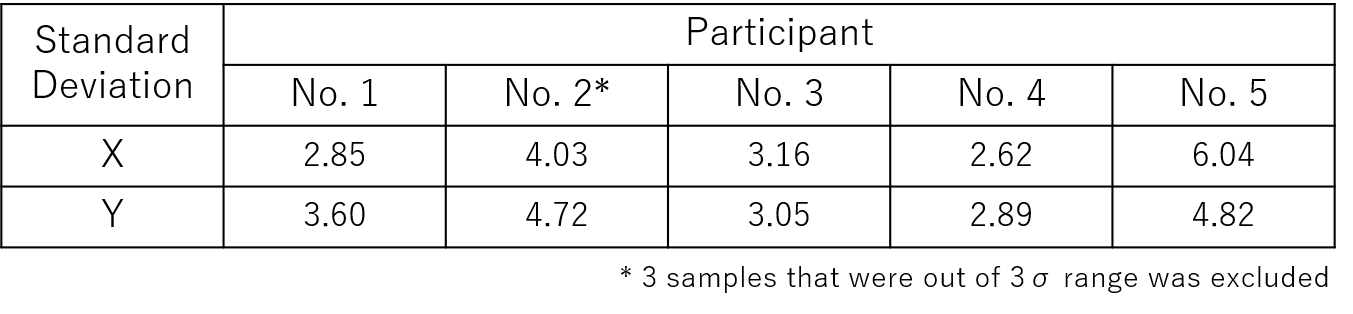
\includegraphics[width=3.2in]{images/tbl_ex2_res}
  \label{tbl_ex2_res}
\end{table}

We removed three outlier samples that were out of a 3$\sigma$ range.
All of the removed samples were the ones obtained from participant No.2.
We plot the compensated value of each participant when the center of friction field was (0,0) in Fig.\ref{fig_ex2_res}.
% In all participants except the participant 2, the center coordinates of the fingertip were located in a friction field with a radius of 20 mm in all trial. 

% The center coordinate of the fingertip varies depending on individual differences, time, and circumstances.
% In order to correct these differences, the mean value of the responses of each participant was taken as the center coordinates of the participant's fingertip, and a value obtained by subtracting the coordinates of the participant's fingertip from each answer value of the participant was taken as the compensated value.

Table.\ref{tbl_ex2_res} shows the standard deviation of along $X$ and $Y$ axes for each participant. 
%According to the t-test, there is a significant difference in standard deviation between $X$ and $Y$ axes for only participant No.2 ($p<0.01$).
According to the t-test result in standard deviation between $X$ and $Y$ axes, there was no significant difference other than No.2 ($p<0.01$).

\subsection{Discussion}

The results show that participants accurately recognized the position of the friction field (Fig.\ref{fig_ex2_res}).
And, the standard deviation represents the error of the participant fingertip's $X$ and $Y$ coordinates from the center of the friction field.
The error between true center position and the answered position were varied from participant to participant (Table.\ref{tbl_ex2_res}).

According to the t-test result, the difference in error along $X$ and $Y$ axes are significant for participant No.2.
This suggested the effect of shear force distribution feedback to users.
The participants were able to determine the center based on the distribution of shear force feedback by moving his finger in the X-axis direction.

%指をx軸方向に揺さぶりながらy軸方向に進めることで,y軸方向の摩擦分布を理解可能
%x, y軸の標準偏差に差が見られなかった原因かも
In contrast, there were no significant differences for other participants'{} data.
One of the reason of the result is that participants were able to recognize the center along the $ Y $ axis with the help of the $ X $ axis shear force feedback.
First, participants recognized the intensity of the local friction at a certain point by shaking their finger along the $X$ axis.
Then, participants moved their finger along $Y$ axis and compared the intensity of local friction along $Y$ axis.

% In this experiment, it was possible to understand the friction distribution in the $Y$ axis direction by moving the finger in the $Y$ axis direction while shaking the finger in the $X$ axis direction.
% Therefore, it is considered that there was no significant difference in the standard deviation between the $X$ axis and the $Y$ axis direction.

%One of the reason why there was no significant difference is that the task was easy and thus, normal indentation was enough to recognize the center position.

We are considering two plans as future work. 
The first plan is to make the contact point denser by miniaturization of the pins.
The second plan is to increase the degree of freedom that the device can present the stimulus. 
Currently, this device is possible to present the 2-DoF direction of the finger. In addition to this, we plan to add one more DoF by increasing the number of pins of 1 pair to 3, aiming at interaction with more natural objects.



% Considering that the distance between the pins of the device is 3.0 mm, the standard deviation of participants No.1, No.3 and No.4 were close to the distance between the pins.
% This indicates the possibility that participants 1, 3 and 4 were able to recognize the change in force output from the pair pins that tilted to the right and the left arranged at $3 \times 3$. 
% However, it has been confirmed that the stimulus shift discrimination threshold is 10 to 30 times smaller than the 2-point discrimination threshold when the stimuli shifts [9]. 
% Considering that the 2-point discrimination threshold of the human fingertip is 2mm to 3mm [15], it can be seen that there is a large gap between the variation from the center of the friction field obtained in this experiment and the stimulus shift discrimination threshold. 
% In addition, there is a mismatch in the action point of the left and right stimulus of this device, so that there is a possibility that the sense of discomfort might disturb the recognition of the subject. 

% \section{LIMITATION}

% 一方、異なるピンの作用点を完全に一致させることはできない。
% この作用点のずれはモーメント(ひねりの成分)を生じることが懸念される。

\section{CONCLUSIONS}

This study proposes a novel method of presenting force distribution in various direction with fixed pin-array display, in which pins are tilted.
We present users with the resultant force by summing up the individual forces from pins which tilted differently.
We hypothesize that we can control the felt direction of resultant force by only changing the air pressure applied to each pin.
We made 45$^{\circ}$ device and 60$^{\circ}$ device to prove the concept.
With this system, we conducted the Experiment 1 on  how well users can discriminate the direction of the resultant force.
JND, which is the discrimination threshold of each device, was 43.3$^{\circ}$ for the 45$^{\circ}$ device and 39.6$^{\circ}$ for the 60$^{\circ}$ device.
In addition, we conducted the Experiment 2 to investigate whether users could find a force field resorting to frictional force distribution applied by the device.
The results show that participants were able to estimate the position of the virtual friction field on the basis of force distribution from the device.
% However, the variation from the center point of friction field was larger than fingertip stimulation shift discrimination threshold.


%%%%%%%%%%%%%%%%%%%%%%%%%%%%%%%%%%%%%%%%%%%%%%%%%%%%%%%%%%%%%%%%%%%%%%%%%%%%%%%%

\addtolength{\textheight}{-12cm}   % This command serves to balance the column lengths
                                  % on the last page of the document manually. It shortens
                                  % the textheight of the last page by a suitable amount.
                                  % This command does not take effect until the next page
                                  % so it should come on the page before the last. Make
                                  % sure that you do not shorten the textheight too much.

%%%%%%%%%%%%%%%%%%%%%%%%%%%%%%%%%%%%%%%%%%%%%%%%%%%%%%%%%%%%%%%%%%%%%%%%%%%%%%%%



%%%%%%%%%%%%%%%%%%%%%%%%%%%%%%%%%%%%%%%%%%%%%%%%%%%%%%%%%%%%%%%%%%%%%%%%%%%%%%%%



%%%%%%%%%%%%%%%%%%%%%%%%%%%%%%%%%%%%%%%%%%%%%%%%%%%%%%%%%%%%%%%%%%%%%%%%%%%%%%%%


\section*{ACKNOWLEDGMENT}

The University of Electro-Communications Ethics committee approved the data acquisition in this paper and written informed consent was obtained from all participants.

\bibliographystyle{IEEEtran}
\bibliography{bibdata}


\end{document}
